\subsection{تخمین پارامترهای کانال پپچ}
برای اصلاح پارامترهای پپچ چندین آزمایش انجام شد و با استفاده از داده‌های ثبت شده از وضعیت استند در کانال پپچ و جعبه‌ابزار
\lr{Parameter Estimator}،
پارامترهای کانال پپچ اصلاح شدند.
برای انجام آزمایش هر یک از موتورهای دو و چهار  با دور مختلف شروع به حرکت کردند و از خروجی سنسور داده برداری شد. سپس، مدل و داده‌های ثبت شده‌ی سنسور (وضعیت استند در کانال پپچ) به جعبه‌ابزار
\lr{Parameter Estimator}
داده شد. وضعیت کانال پپچ استند در شبیه‌سازی و واقعیت بعد از اصلاح پارامترهای کانال پپچ در شکل‌های
\ref{pitch_ps1}, \ref{pitch_ps2}, و \ref{pitch_ps3}
مقایسه شده است.

\begin{figure}[H]
	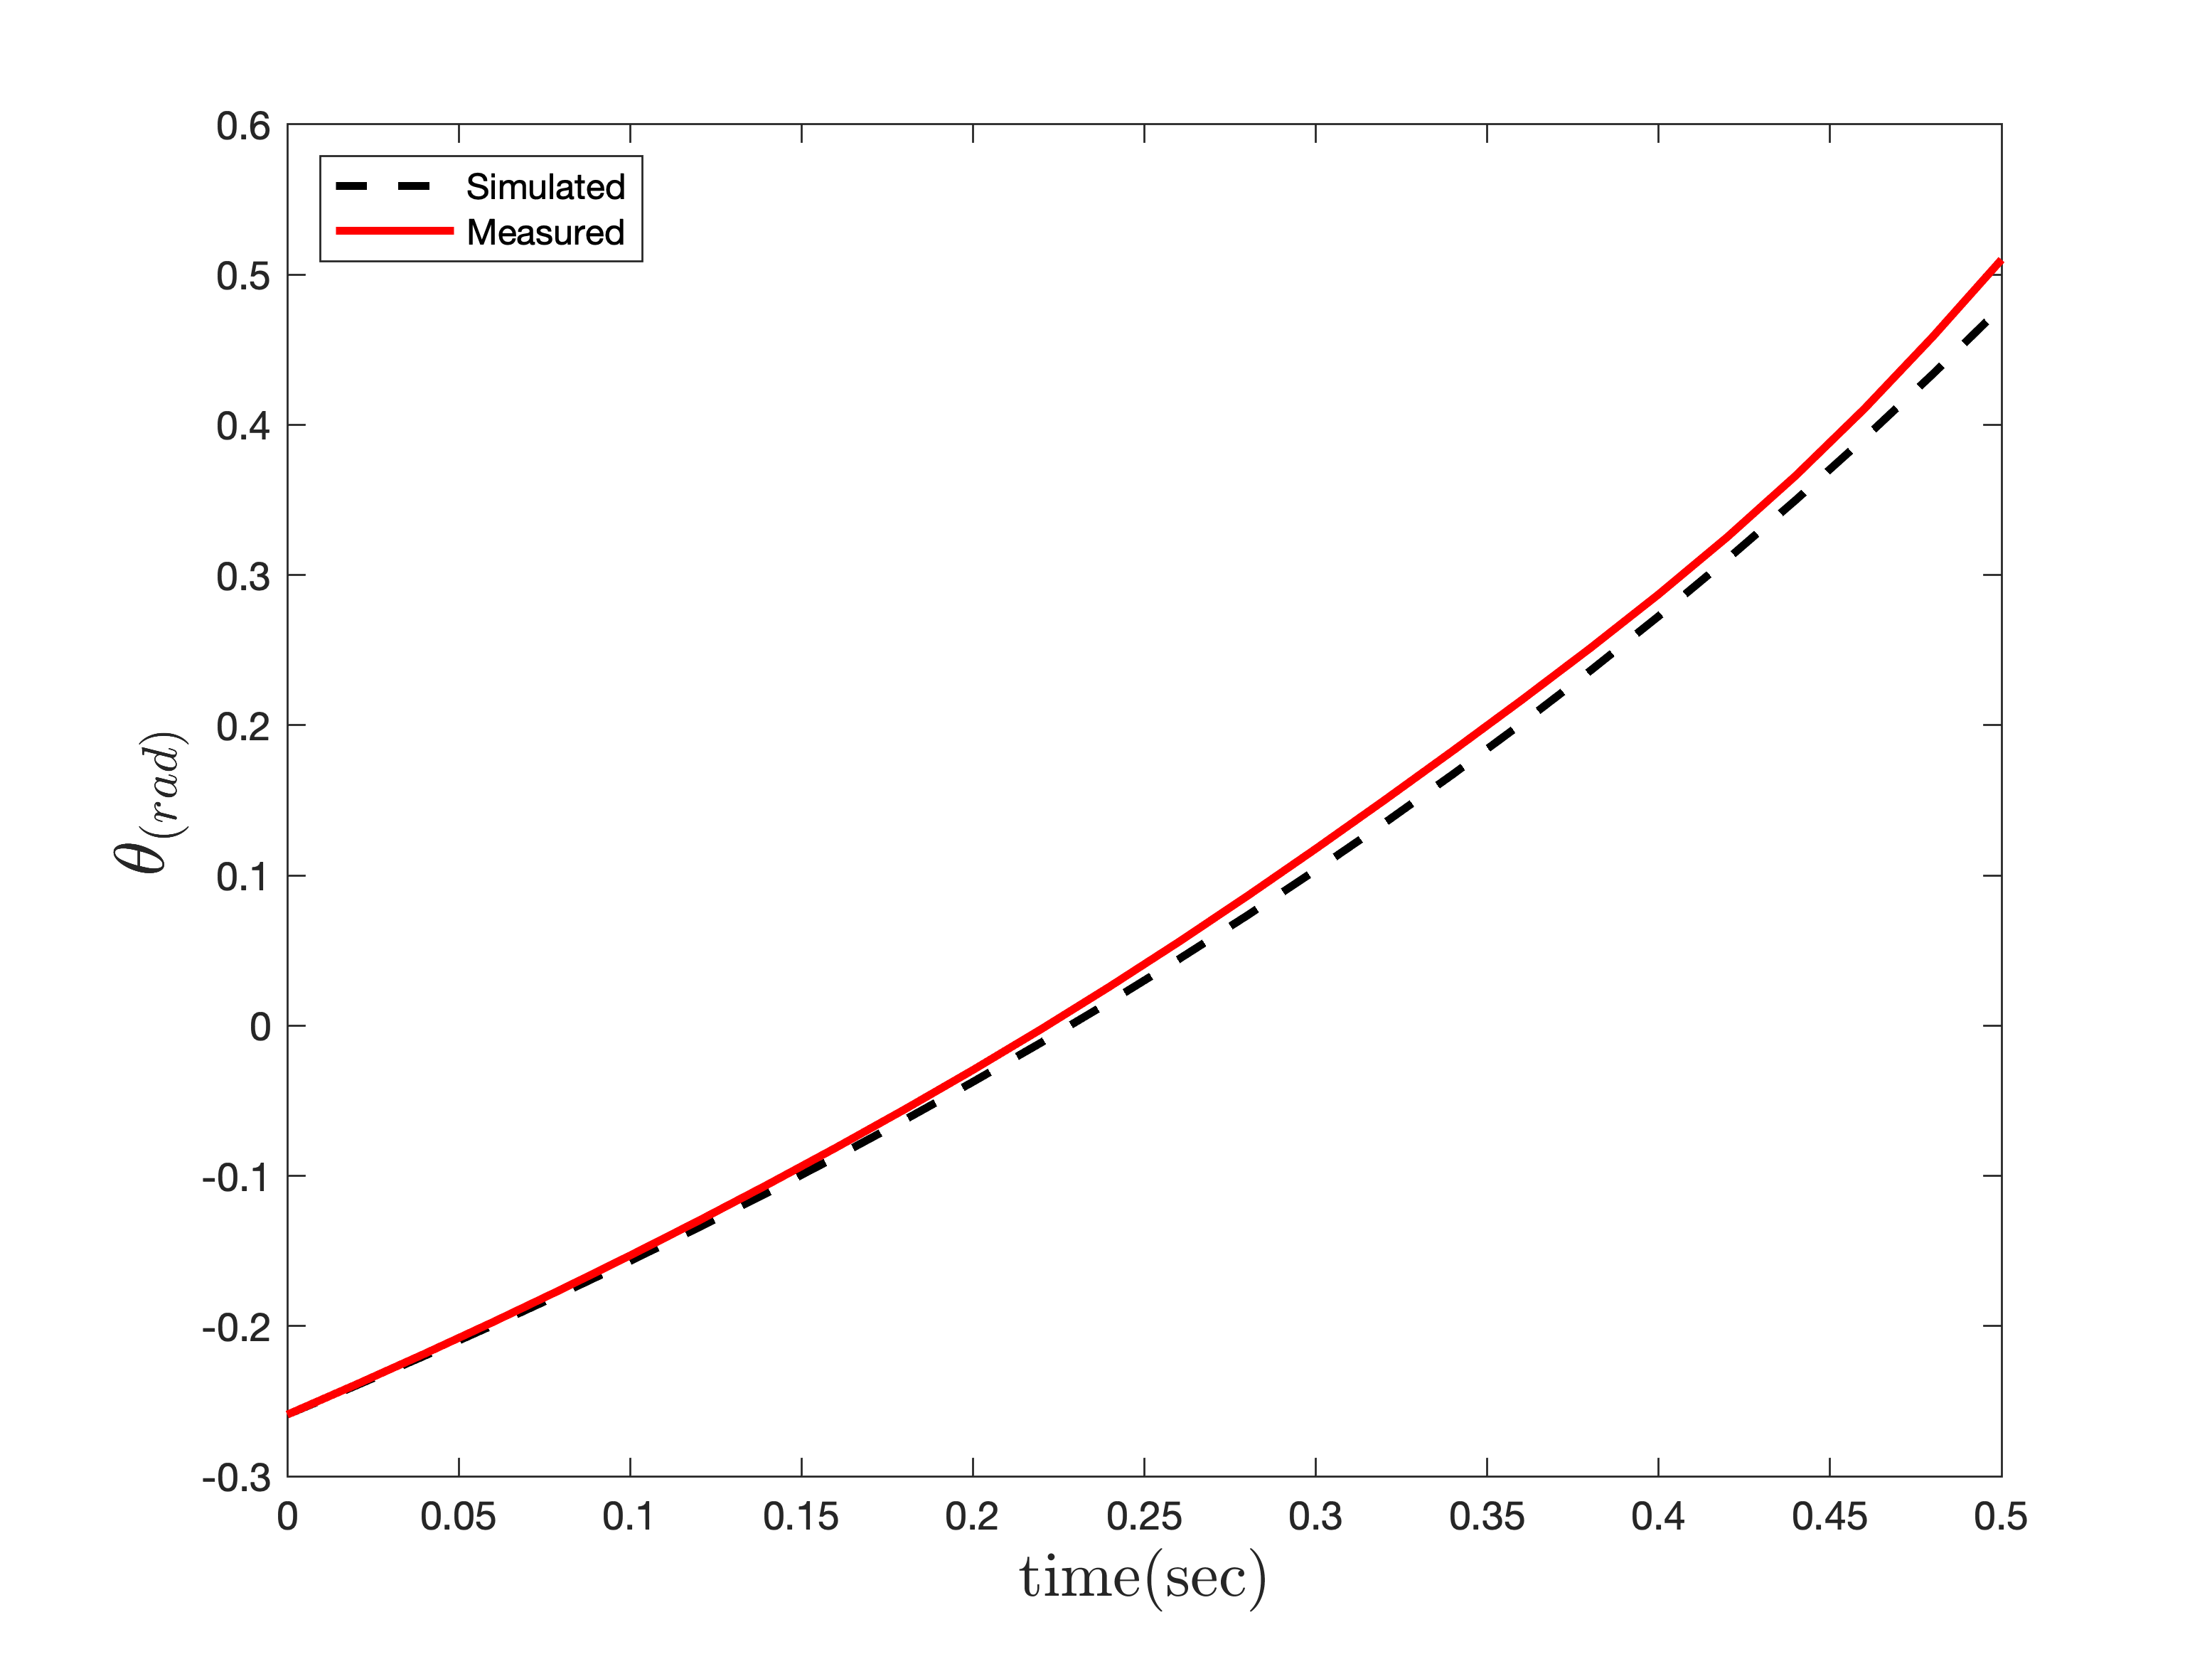
\includegraphics[width=12cm]{../../Figures/RCP/pitch_parameter_estimation/RCP_pitch_S1.png}
	\centering
	\caption{مقايسه وضعیت استند در  آزمايش اول و شبیه‌سازی، پس از تخمین پارامترهای کانال پپچ}
	\label{pitch_ps1}
\end{figure}
\begin{figure}[H]
	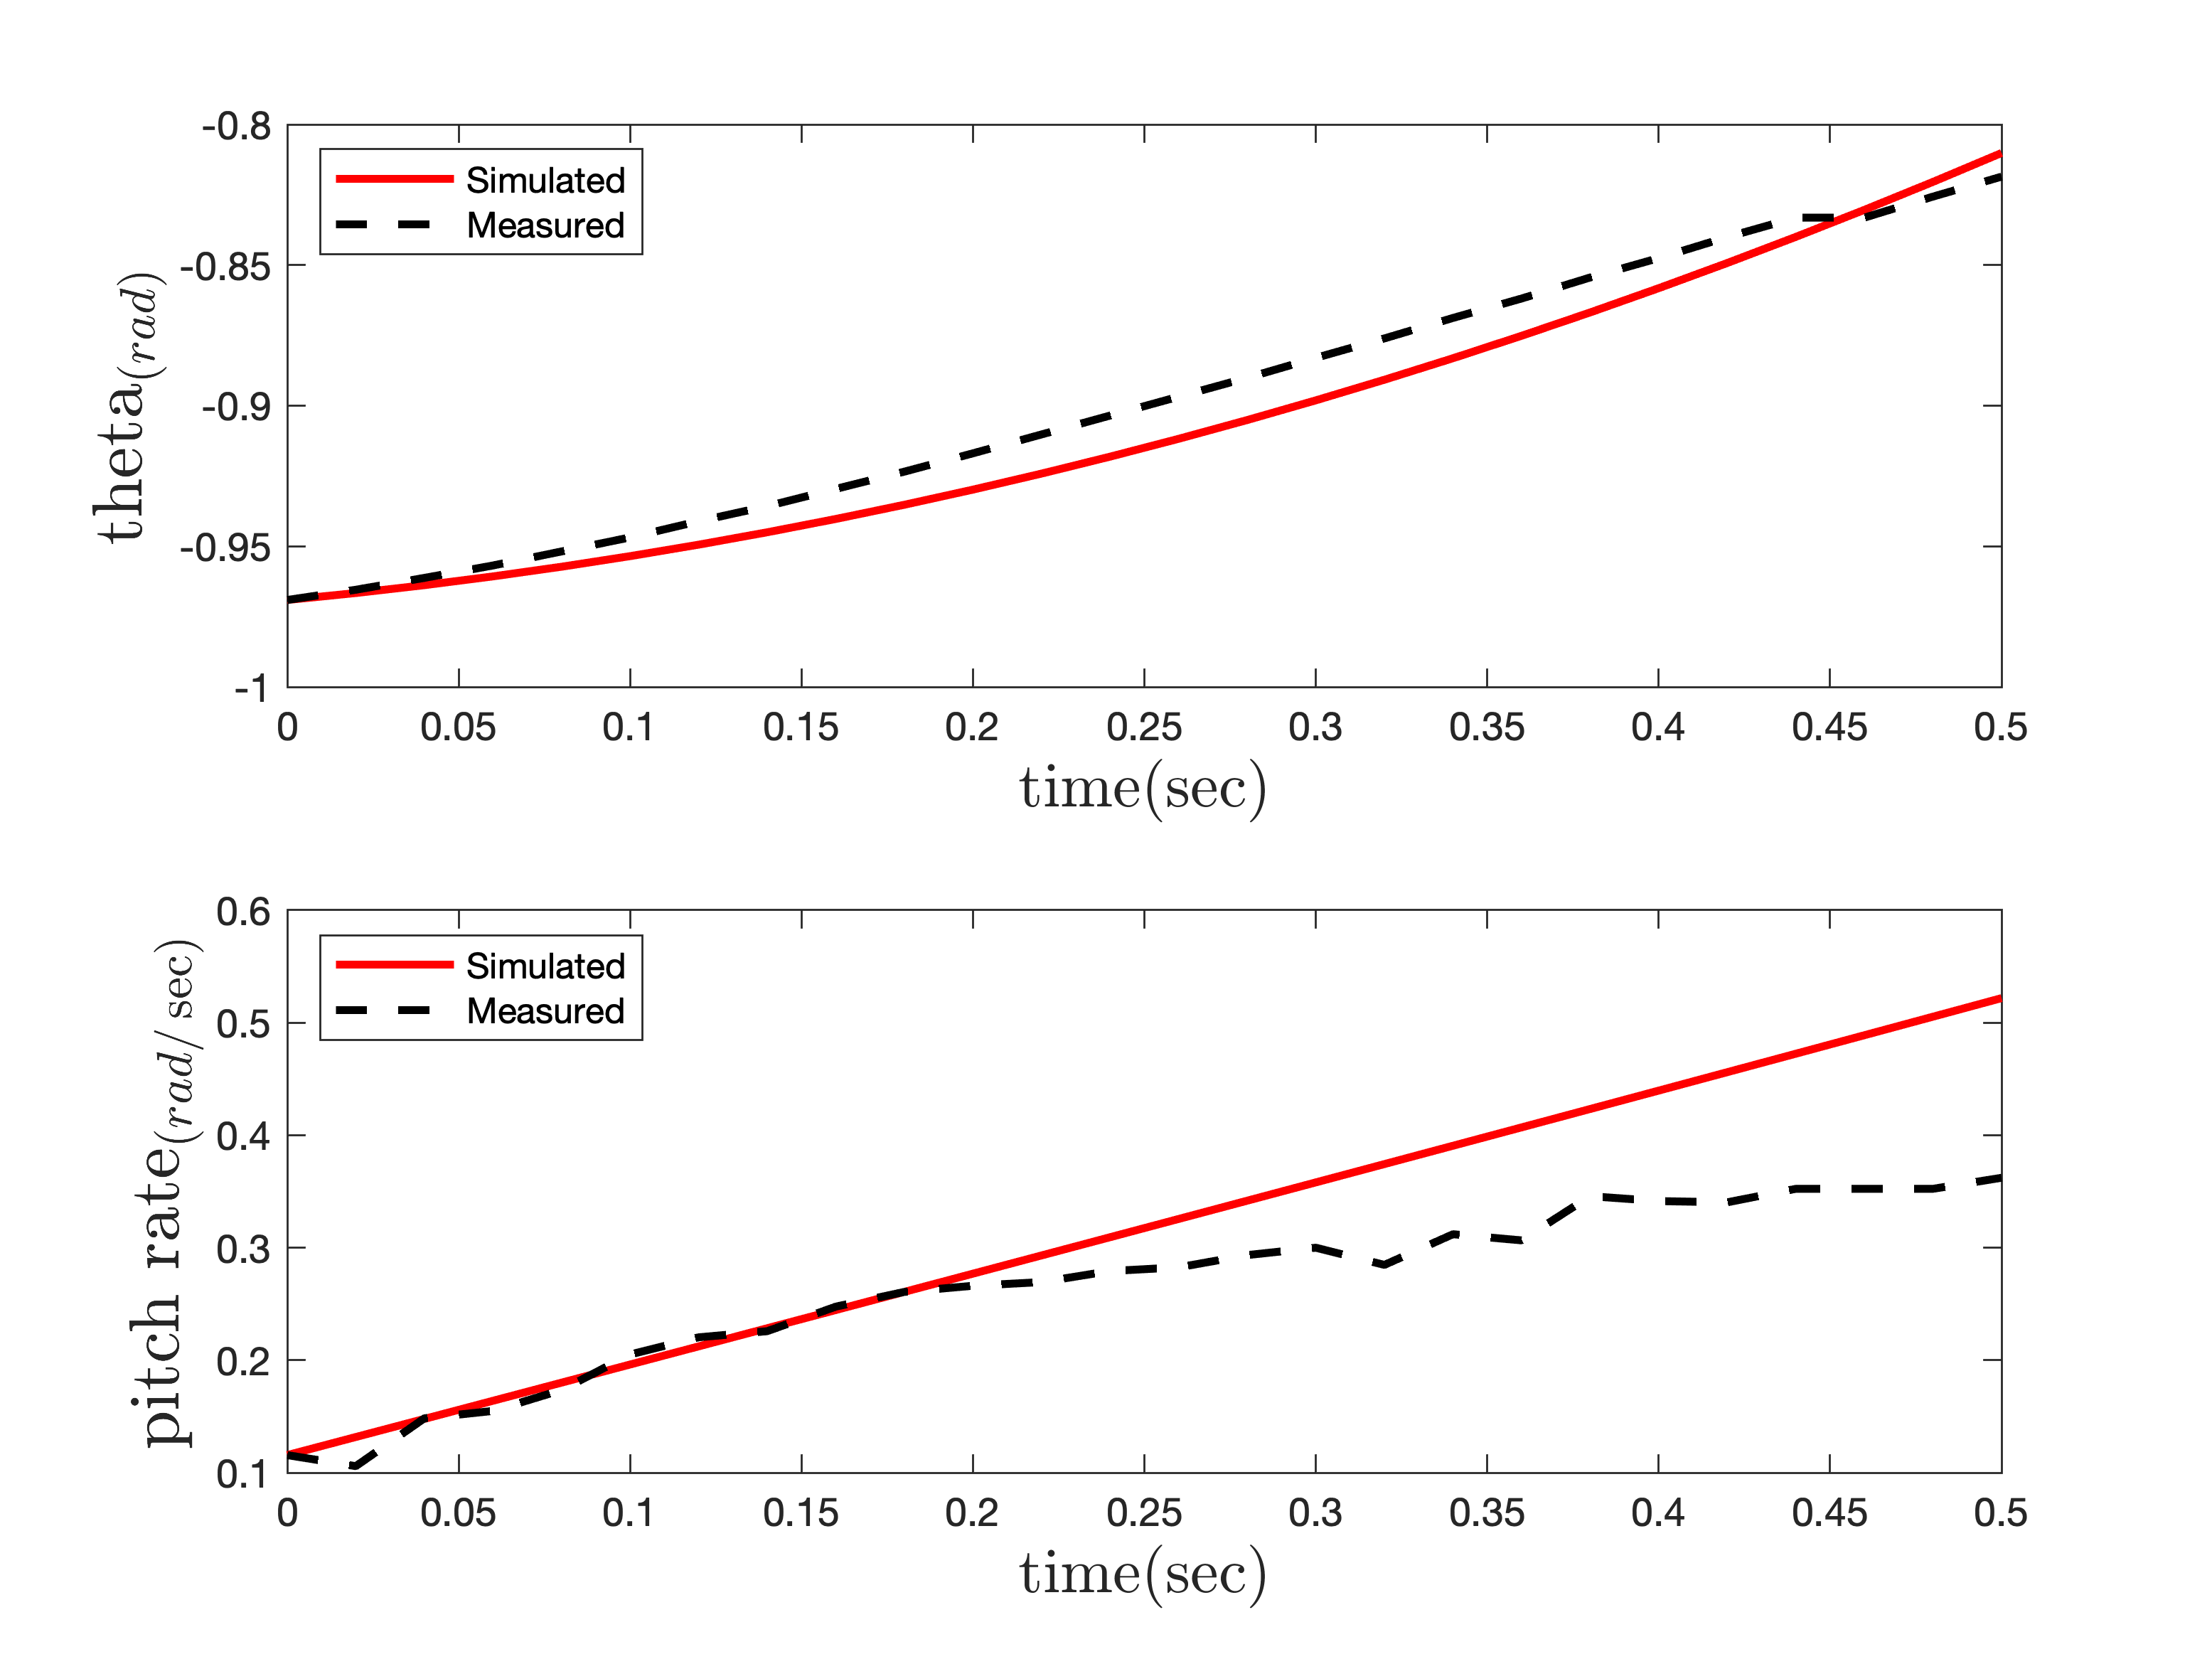
\includegraphics[width=12cm]{../../Figures/RCP/pitch_parameter_estimation/RCP_pitch_S2.png}
	\centering
	\caption{مقايسه وضعیت استند در  آزمايش دوم و شبیه‌سازی، پس از تخمین پارامترهای کانال پپچ}
	\label{pitch_ps2}
\end{figure}
\begin{figure}[H]
	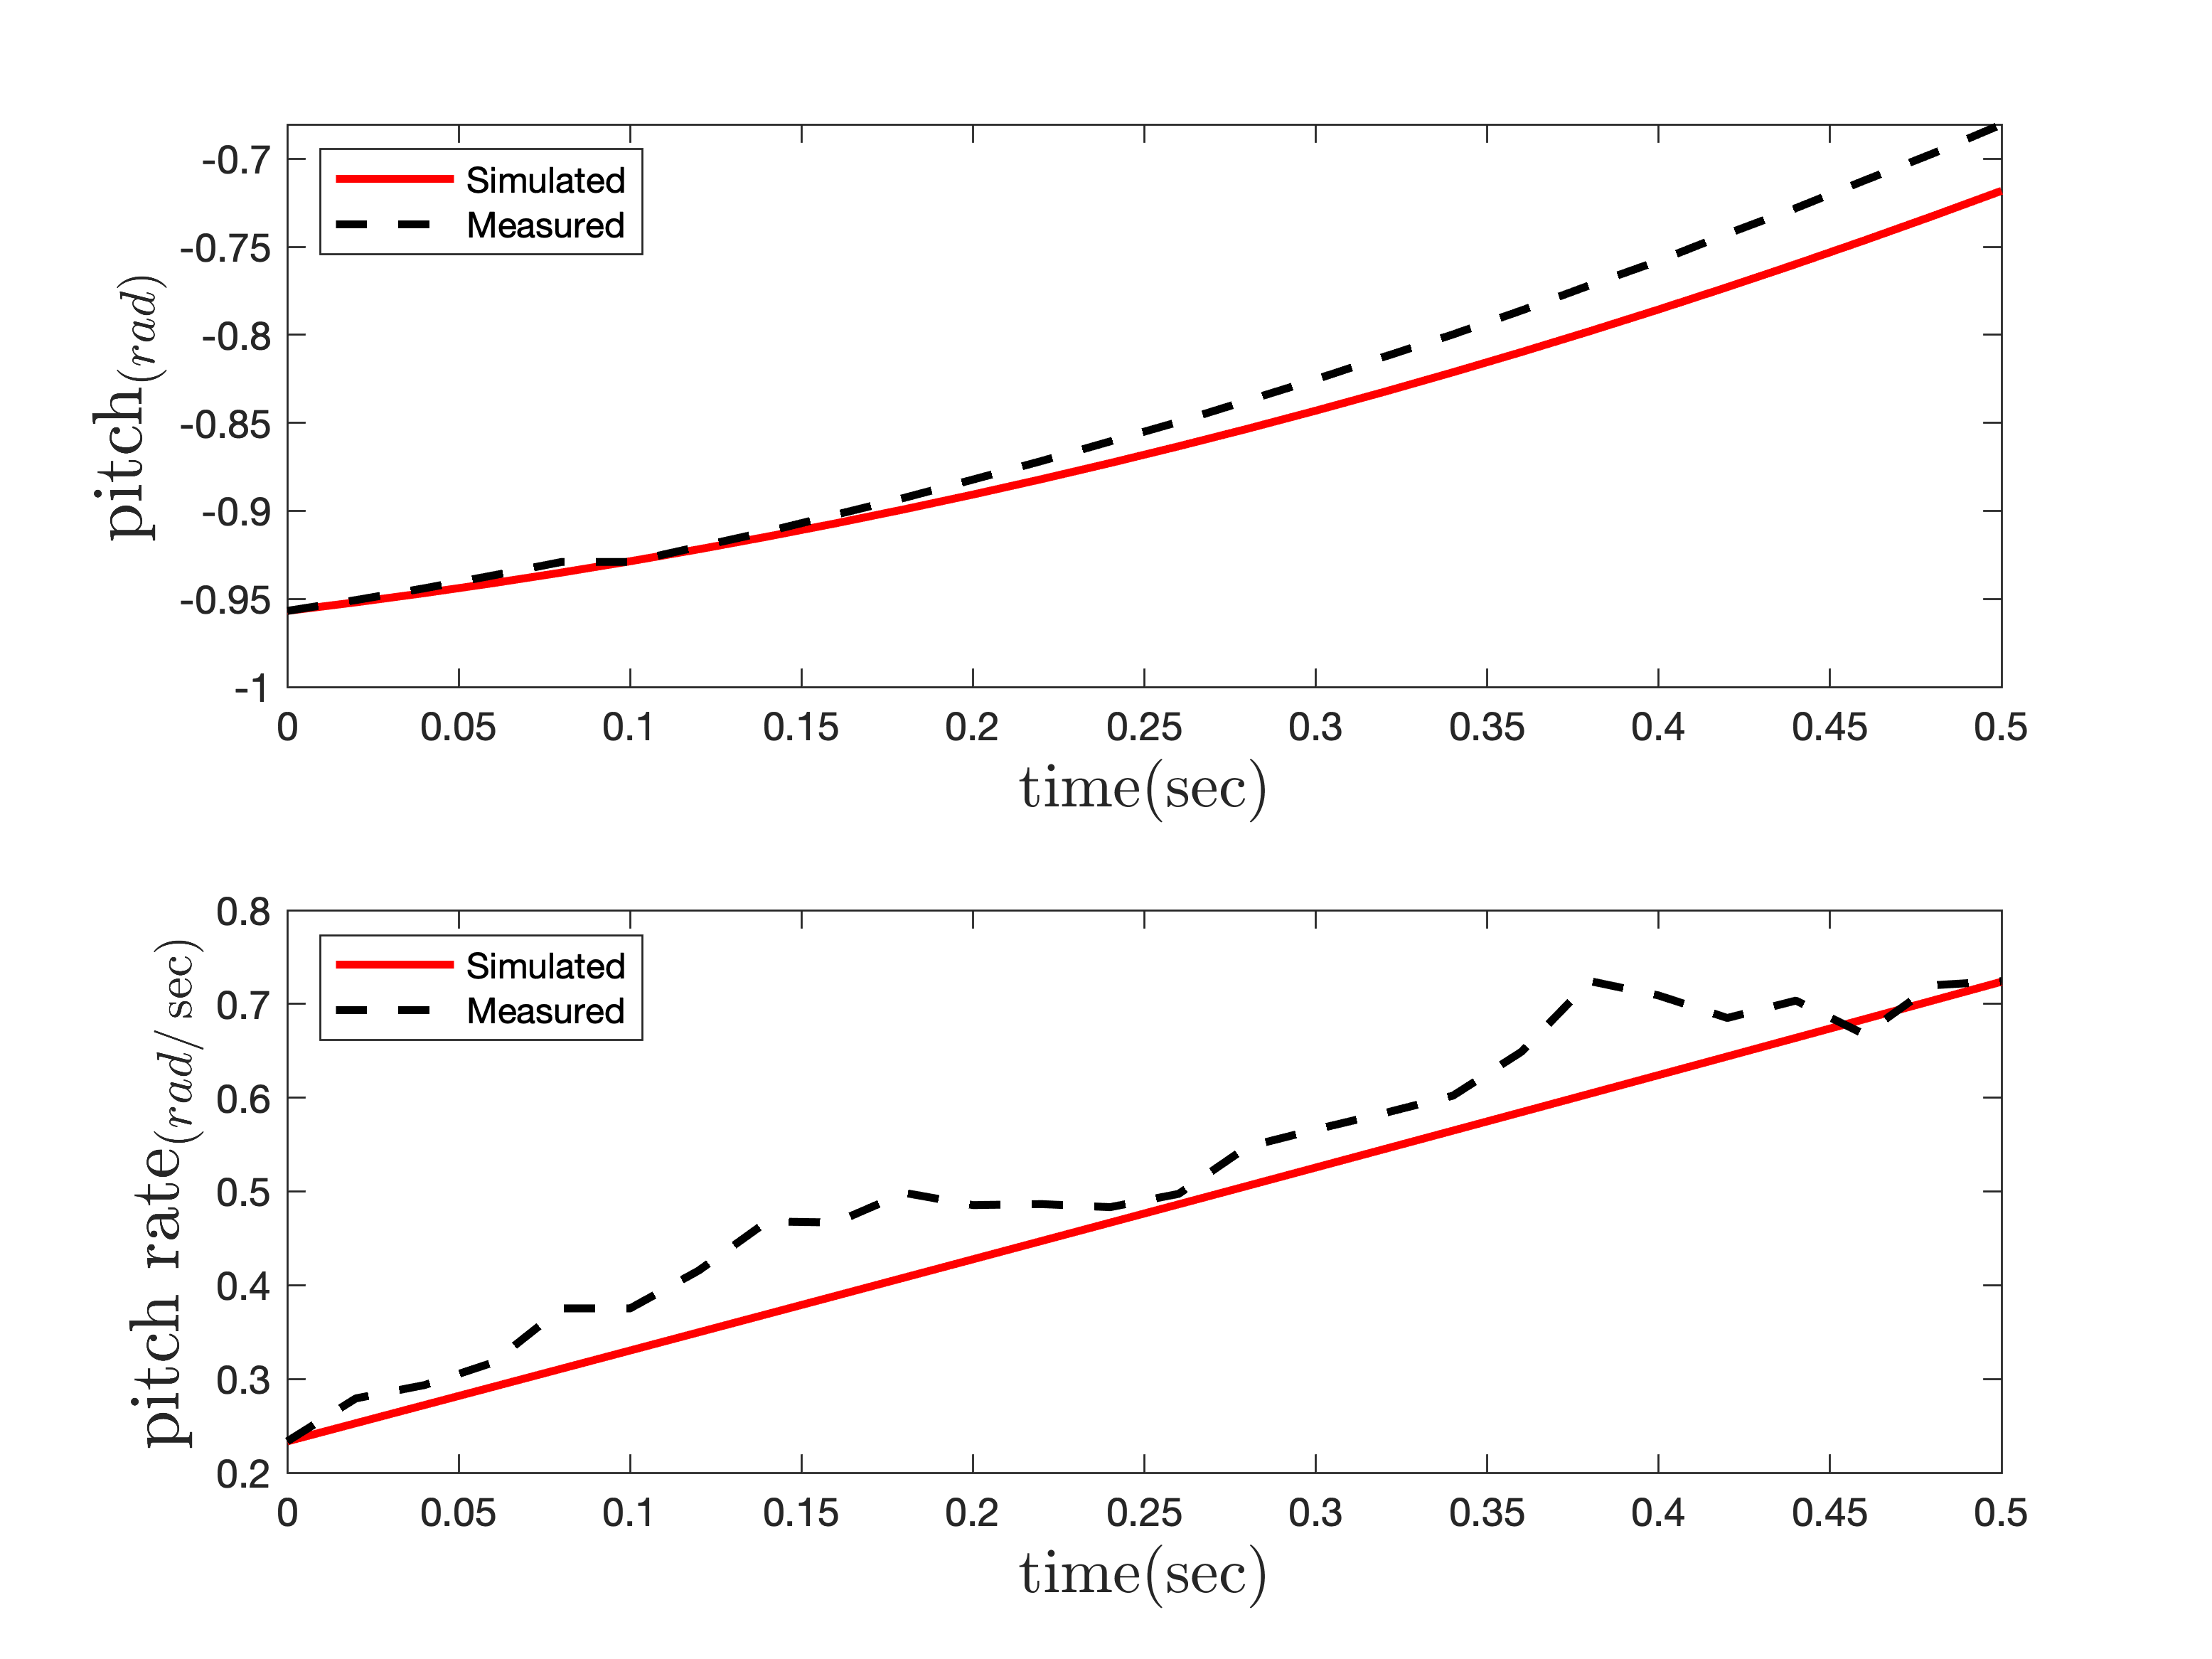
\includegraphics[width=12cm]{../../Figures/RCP/pitch_parameter_estimation/RCP_pitch_S3.png}
	\centering
	\caption{مقايسه وضعیت استند در  آزمايش سوم و شبیه‌سازی، پس از تخمین پارامترهای کانال پپچ}
	\label{pitch_ps3}
\end{figure}
